\chapter{Hot electron temperature models}
In this chapter, we will talk about the models suitable for hot electron temperature modelling. It was already hinted in the first chapter that there are many physical processes contributing to the absorption of laser. As a consequence, there is a non-linear relationship between the initial parameters and the hot electron temperature. It would be very difficult to propose an analytical model where the temperature is explicitly dependant on all the initial parameters. There have been works studying how the temperature scales with respect to intensity \cite{kluge2011,cui2013,miller2023,haines2009,beg1997}, angle \cite{cui2013} or length scale and even pulse durations \cite{miller2023}, but none of them models the dependency on all parameters at once. Needless to say, these works are valuable and they will be discussed with respect to predictions of our final model in chapter \ref{ch:comparison}.

Given the complexity and multi-dimensionality of our dataset, few machine learning regression methods offer a promising alternative to analytical models. We will now discuss general principle of regression and several particular regression methods as well as their suitability for this thesis based on previous works.

\section{Regression methods}
Regression is a fundamental technique in machine learning used for predicting continuous outcomes \cite{bishop2006}. Formally, for the set of data $D = \left\{(\bm{x_1},y_1),...,(\bm{x_n},y_n)\right\}\in \mathcal{X}\times\mathbb{R}$, where $\mathcal{X}$ is $d$-dimensional space of inputs, we want to find a function $f(\bm{x},\bm{w})$ that represents the relationship between $\bm{x}_i$ and $y_i$. $\bm{w} = (w_0,..,w_{m})$ is the vector of parameters of $f$. In the observations, we assume a Gaussian noise with zero mean and variance $\sigma^2$ so we can write:
\begin{equation}
	y_i = f(\bm{x_i},\bm{w}) + \epsilon_i,
\end{equation}
where $\epsilon_i \sim \mathcal{N}(0,\,\sigma^{2})$ is the noise.

Moreover, we want the function $f(\bm{x},\bm{w})$ to be able to generalize - to give accurate predictions for inputs not present in the training dataset. A good regression process balances the trade-off between fitting the training data accurately and maintaining predictive performance on unseen data. This condition transforms most regression problems to an optimization problem, where one tries to find the best model under certain conditions.

A good example is generalized linear regression where the model is given by:
\begin{equation}
	\label{eq:gen-linear-model}
	y = w_0 + \sum_{i=1}^{m}\phi_i(\bm{x})w_{i} = \bm{w}^T\bm{\phi}(\bm{x})
\end{equation}
where $\phi_i(\bm{x})$, $i=1,..,m$ are transformation functions of the inputs also called \textit{basis functions} and $\phi_0(\bm{x})=1$ \cite{bishop2006}. A reasonable metric of the goodness of this model (sometimes also called \textit{loss}) can be the sum of square of errors ($SSE$) calculated on dataset:
\begin{equation}
	SSE(\bm{w}) = \frac{1}{2}\sum_{i=0}^{n}\left(\bm{w}^T\bm{\phi}(\bm{x_i})-y_i\right)^2
\end{equation}
Minimizing $SSE$ with respect to weights in simple problems with correctly chosen $\bm{\phi}$ is often enough to get a reliable predictor. This usually requires a good knowledge about the data. If the model is over-fitted - $SSE$ is small for training data but large for new data - modifying the error function might help. For example, one can add $regularization$ term $\frac{\lambda}{2}\bm{w}^T\bm{w}$ to the $SSE$. This introduces \textit{hyper-parameter} $\lambda$, which controls the importance of weights being small. The loss function to minimize is:
\begin{equation}
	SSE_{\mathrm{reg}}(\bm{w}) = \frac{1}{2}\sum_{i=0}^{n}\left(\bm{w}^T\bm{\phi}(\bm{x_i})-y_i\right)^2 + \frac{\lambda}{2}\bm{w}^T\bm{w}
\end{equation}
Minimizing $SSE_{\mathrm{reg}}$ instead of $SSE$ sometimes helps complex models to improve their predictive performance \cite{bishop2006}.

The optimization problem can be reversed to so called maximum likelihood estimation (MLE), where instead of minimizing an error function, one tries to find model maximizing the probability that we observe data given the set of parameters. In case of Gaussian noise, this approach is equivalent to minimizing $SSE$ \cite{bishop2006}.


The appropriate selection of the feature mapping $\bm{\phi}$ enables one to effectively capture non-linear relationships. However, in situations where determining the exact form of $\bm{\phi}$ is ambiguous, various methodologies have been developed to accommodate modelling without explicit knowledge of the underlying model structure. In the following sections, we look into advanced techniques for non-linear regression. We begin with Support Vector Regression (SVR), followed by a brief overview of Neural Networks, and finally, a more detailed exploration of Gaussian Processes.

\section{Support vector regression}
Support vector regression (SVR) is powerful regression technique capable of modelling non-linear relationship without any previous assumption about the model. From its formulation it is directly set up to balance complexity and prediction error~\cite{zhang2020}. In several following paragraphs, we will present the most important principles of SVR.

\subsection*{Linear $\epsilon$-SVR model}
Assuming simple linear model we can simplify equation \ref{eq:gen-linear-model} to $y = \bm{\bar{w}}^T\bm{x} + w_0$ where $\bm{\bar{w}} = (w_1,..,w_d)$. In $\epsilon$-SVR, there are constraints put on the predictions in such way that the prediction $ \bm{\bar{w}}^T\bm{x_i} + w_0$ cannot be further from $y_i$ than $\epsilon$. We also want the \textit{tube} defined by $\epsilon$ to be as \textit{flat} possible, which can be done by minimizing $\frac{1}{2} \bm{w}^T\bm{w}$~\cite{zhang2020}.

In reality, having rigid boundary at distance $\epsilon$ from $y_i$ is not practical because of outliers. It is therefore natural to introduce two $slack$ variables $\xi_i$ and $\xi_i^*$, which are used to widen the tube at the points of observation. The optimization problem can be formulated as \cite{smola2004}:
\begin{align}
	\label{eq:svr1}
	\mathrm{minimize}\qquad & \frac{1}{2}\bm{w}^T\bm{w} + C\sum_{i=1}^{n}\left(\xi_i+\xi_i^*\right)  \\
	\mathrm{subject}\,\mathrm{to}\qquad & 
	\begin{dcases} 
		\label{eq:svr2}
		y_i - (\bm{\bar{w}}^T\bm{x}_i + w_0) 	& \leq \epsilon + \xi_i \\ 
		(\bm{\bar{w}}^T\bm{x}_i + w_0) - y_i  & \leq \epsilon + \xi_i^* \\
		           \xi_i,\,\xi_i^*   		& \geq 0 
	\end{dcases}
\end{align}

\subsection*{Kernel SVR}
By so-called \textit{kernel trick} - transforming features $\bm{x}_i$ to a higher-dimensional kernel space $\mathcal{F}$, we can leave the assumption that the relationship between $\bm{x}$ and $y$ is linear. Let us note the mapping $\phi(\cdot): \mathcal{X} \rightarrow \mathcal{F}$. $\bm{x}_i$ in \ref{eq:svr1} and \ref{eq:svr2} is replaced by $\phi(\bm{x})$. Moreover, the new optimization problem can be written in dual form \cite{smola2004}:
\begin{equation}
	\mathrm{max}_{\alpha_i,\alpha_i^*} \; -\frac{1}{2}\sum_{i,j}^{n}\left(\alpha_i - \alpha_i^*\right)\left(\alpha_j - \alpha_j^*\right)k(\bm{x}_i,\bm{x}_j) -\epsilon\sum_{i}^{n}\left(\alpha_i + \alpha_i^*\right) + \sum_{i}^{n}y_i\left(\alpha_i - \alpha_i^*\right)
\end{equation}
\begin{equation}
	\mathrm{subject}\,\mathrm{to}\quad  \sum_{i}^{n}\left(\alpha_i - \alpha_i^*\right) \,\mathrm{and}\, \alpha_i, \alpha_i \in \left[0,C\right]
\end{equation}
where $k(\bm{x}_i,\bm{x}_j) = \phi(\bm{x}_i)\phi(\bm{x}_j)$ is the kernel function. There are multiple conditions which the kernel function must satisfy and they can be found in \cite{smola2004}. Popular kernels include linear, polynomial, radial basis function and others \cite{zhang2020}.
Note that $\bm{w}$ is no longer explicitly present. Another important fact is that in this case, the flatness is important in the new space $\mathcal{F}$ and not the original input space $\mathcal{X}$ \cite{smola2004}.

To determine the hyper-parameters $\epsilon$ and $C$ (or other parameters associated with the kernel itself), it is customary to perform a \textit{cross-validation} where we randomly divide the dataset to two parts - training set and test set - and evaluate the predictive performance only on the latter which is not used during the optimization \cite{zhang2020}.

\section{Neural networks}
Neural networks have a different approach. They still assume almost nothing about the modelled relationship, but as opposed to SVR, where the goal is to minimize the confidence interval by searching for a flat solution, neural networks usually search directly for minimum error on the training data \cite{vapnik2000}. 

The simplest neural network is probably the  Multilayer Perceptron (MLP). A MLP is a type of neural network that consists of an input layer, one or more \textit{hidden} layers, and an output layer. Each layer is composed of neurons, and each neuron in a layer is connected to every neuron in the subsequent layer. Neuron linearly combines all the outputs from the previous layer using its own set of weights and then transforms the result to its output using some function. The mathematical formulation of an MLP can be described as follows:

1. \textbf{Input Layer:} Let the input vector be $\bm{x}$.

2. \textbf{Hidden Layers:} Consider a single hidden layer with $m$ neurons. The output of the $j$-th neuron in the hidden layer, denoted as $h_j$, is given by:
\begin{equation}
	h_j = \sigma\left( \sum_{i=1}^{n} w_{ij}^{(1)} x_i + b_j^{(1)} \right)
\end{equation}
where $w_{ij}^{(1)}$ is the weight connecting the $i$-th input to the $j$-th hidden neuron, $b_j^{(1)}$ is the bias term for the $j$-th hidden neuron, and $\sigma$ is the \textit{activation function}, that introduces non-linearity.

3. \textbf{Output Layer:} Let the output layer have $1$ neuron. The output of the $l$-th neuron in the output layer, denoted as $y_l$, is given by:
\begin{equation}
	y_l = \phi\left( \sum_{j=1}^{m} w_{jl}^{(2)} h_j + b_l^{(2)} \right)
\end{equation}
where $w_{jl}^{(2)}$ is the weight connecting the $j$-th hidden neuron to the $l$-th output neuron, $b_l^{(2)}$ is the bias term for the $l$-th output neuron, and $\phi$ is the activation function for the output layer (for regression $\phi$ is the identity) \cite{bishop2006}.

Note that for each layer weights are well represented as matrix. Number of hidden layers and the number of neurons has to be chosen. However, even with only two layers with linear outputs, any continuous function on a compact domain can be approximated to arbitrary precision if the total number of neurons is large enough~\cite{bishop2006}.

\subsection*{Training the MLP}
The training of neural network includes usually calculating gradients of the loss function with respect to the weights, propagating the gradients back through the network and updating the weights - also knows as \textit{gradient descent}. It is usually the case that if the loss and the activations are differentiable functions (w.r. to the weights), because their derivative is needed for the error back-propagation \cite{bishop2006}.

Gradient descent alone can find local minimum of the error function for the training data but it says nothing about the ability to recognize patterns. There are multiple \textit{regularization} strategies that help neural network generalize but in contrast to SVR they have to be fine-tuned. Common ones are early stopping (not letting the weights to come to the local minimum completely), weight decay (e.g. using $SSE_{\mathrm{reg}}$), batch normalization (the gradients are averaged for multiple training points), or dropout (in each learning process iteration we exclude few neurons from the network) \cite{bishop2006,srivastava2014}.

When training complex non-linear relationship on small datasets (up to 1000 samples), it can be the case that the complexity cannot be captured by network with less weights than the number of training points. This is called \textit{over-parametrization}. However, it is sometimes still valid to train such network, because the effective number of degrees of freedom can be lowered by regularization \cite{barlett1998,ingrassia2005}. Tuning over-parametrized NNs is more difficult, but seeing its predictions side by side with other models can give us a better insight into the properties of our data.

\section{Gaussian Processes}
Another viable regression method is Gaussian Process regression. Its approach is completely different compared to both previous methods. Following paragraphs are explaining the basics of Gaussian Processes.

Gaussian Process (GP) can be understood as an extension of multivariate Gaussian distribution over vectors to distribution over functions. Informally, we replace $\mathcal{N}(\bm{\mu},\bm{\Sigma})$, where $\bm{\mu}$ is mean and $\bm{\Sigma}$ is the covariance matrix, with Gaussian Process $\mathcal{GP}(m(\bm{x}),k(\bm{x},\bm{x}^\prime))$, where $m(\bm{x})$ is mean function and $k(\bm{x},\bm{x}^\prime)$ is covariance function. $m(\bm{x})$  and $k(\bm{x},\bm{x}^\prime)$ fully specify a Gaussian process. For every input $\bm{x}$ there is now a random variable $f(\bm{x})$ for which we can write \cite{rasmussen2004}:
\begin{equation}
	\label{eq:gp}
	f\sim\mathcal{GP}(m(\bm{x}),k(\bm{x},\bm{x}^\prime)).
\end{equation}

Function $k$ is commonly called $kernel$ function as in SVR. Sampling from $f$ can then be done easily, if we know $k$ and $m$ and if we realize that we can usually represent sample function by finite amount of points. 

\begin{figure}[ht]
	\centering
	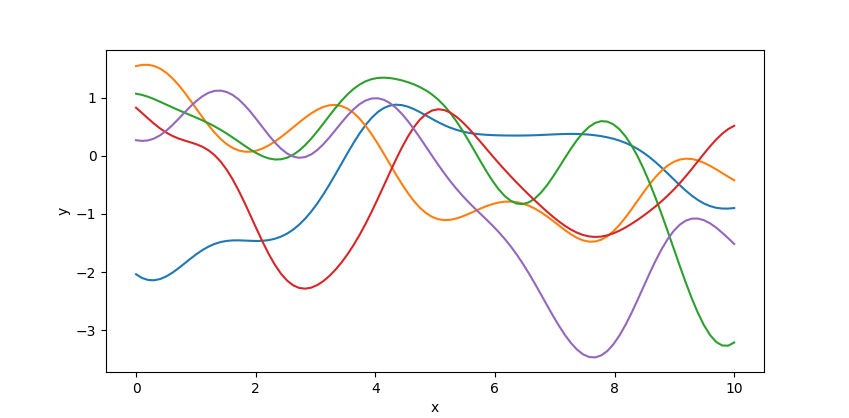
\includegraphics[width=0.98\textwidth]{figures/gaussian-samples}
	\caption{5 sample functions from $\mathcal{GP}(0,\exp(-\frac{(x-x^\prime)^2}{2}))$. It was sampled at 100 points between $x = 0$ and $x=10$.}
	\label{fig:gaussian-samples}
\end{figure}

For sampling, we first calculate covariance matrix $\Sigma_{i,j} = k(\bar{x}_i,\bar{x}_j)$ for points $\bm{\bar{x}} = (\bar{x}_1,.. ,\bar{x}_s)$, at which we want to plot the sampled functions. Each sample is then a vector of size $s$ given by multivariate Gaussian distribution with covariance matrix $\bm{\Sigma}$. As an example, 5 samples from Gaussian Process with $m(x) = 0$ and $k(x,x^\prime) = \exp(-\frac{(x-x^\prime)^2}{2})$ can be seen in figure \ref{fig:gaussian-samples}. Note that the smoothness is a consequence of the choice of the kernel function.

The next step is to update the $\mathcal{GP}$ with the measured data. In other words, we want to condition $f$ from \ref{eq:gp} on dataset $D$. We can write \cite{rasmussen2004}:
\begin{align}
\begin{split}
	\label{eq:gaussian-condition}
	f \vert D & \sim\mathcal{GP}(m_D,k_D) \\
	m_D(\bm{x}) & = m(\bm{x}) + \bm{\Sigma_*(X,x)}^T \bm{\Sigma}^{-1} (\bm{f}-\bm{m}) \\
	k_D(\bm{x},\bm{x}^\prime) & = k(\bm{x},\bm{x}^\prime) - \bm{\Sigma_*(X,x)}^T \bm{\Sigma}^{-1} \bm{\Sigma_*(X,x^\prime)},
\end{split}
\end{align}
where $\bm{\Sigma_*}(X,x)$ is a vector of covariances between every training case $\bm{X}$ and $x\bm{x}$ \cite{rasmussen2004}. Applying equation \ref{eq:gaussian-condition} to our previous example, we can generate new samples from the posterior distribution of functions. The term \textit{posterior} comes from the Bayesian inference. If we let for example the training dataset consist of five points $D = \left\{(1,2),(3,2),(5,3),(7,4),(9,2)\right\}$, the 5 samples from the updated distribution can be seen in figure \ref{fig:gaussian-samples-posterior}.
\begin{figure}[htb]
	\centering
	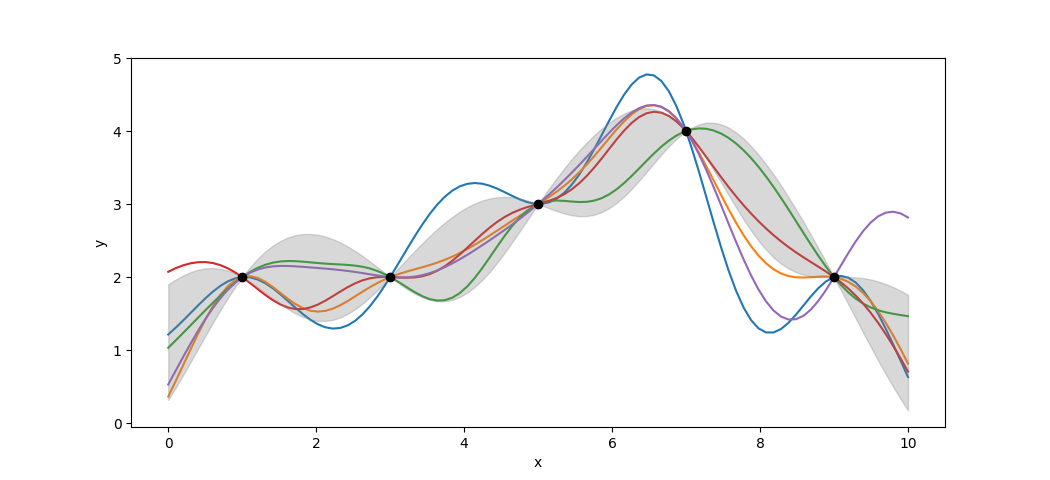
\includegraphics[width=0.98\textwidth]{figures/gaussian-samples-post}
	\caption{5 sample functions from $\mathcal{GP}(m_D,k_D))$. It was sampled at 100 points between $x = 0$ and $x=10$. The grey area depicts one one standard deviation from the mean.}
	\label{fig:gaussian-samples-posterior}
\end{figure}

One can see that the figure \ref{fig:gaussian-samples-posterior} has sample sample functions that go through the points in $D$. This is because that was the condition. A less strict condition would be to set a non-zero noise to the dataset. This allows the samples not to go strictly through all points in the dataset. Mathematically speaking, adding noise is represented by adding a diagonal matrix to the covariance matrix or even more general~\cite{rasmussen2004}:
\begin{equation}
	\begin{split}
		y = f + \epsilon,& \quad  \quad \epsilon \sim \mathcal{N}(0, \sigma_n^2) \\
		f \sim \mathcal{GP}(m(\bm{x}),k(\bm{x},\bm{x}^\prime)), & \quad  \quad y \sim \mathcal{GP}(m(\bm{x}),k(\bm{x},\bm{x}^\prime)+\delta_{xx^\prime}\sigma_n^2),
	\end{split}
\end{equation}
where $\delta_{xx^\prime} = 1$ for $x=x^\prime$ and $\delta_{xx^\prime} = 0$ for $x\neq x^\prime$.

Apart from RBF kernel $k_{\mathrm{RBF}}(x-x^\prime) =\sigma^2\exp(-\frac{(x-x^\prime)^2}{2l})$ another common choice are kernels from the Matern class \cite{rasmussen2005}:
\begin{equation}
	k_\mathrm{Matern}(r) = \frac{2^{1-\nu}}{\gamma(\nu)}\left(\frac{\sqrt{2\nu}r}{l}\right)^\nu K_\nu\left(\frac{\sqrt{2\nu}r}{l}\right),
\end{equation}
where $\nu$ and $l$ are positive paremeters, $r=\norm{\bm{x} -\bm{x^\prime}}$, $\Gamma(\nu)$ is a gamma function and $K_\nu$ is a modified Bessel function. Common choices of $\nu$ are $\frac{1}{2}, \frac{3}{2}$ and $\frac{5}{2}$. For $n \rightarrow \infty$, $k_\mathrm{Matern}(\norm{\bm{x} -\bm{x^\prime}})$ degenerates to $k_{\mathrm{RBF}}(\bm{x} ,\bm{x^\prime})$ \cite{rasmussen2005}.

Gaussian process regression is a non-parametric model, meaning the training data cannot be discarded after the training, because they are needed for the computation of $\bm{\Sigma_*}$. The memory complexity of the algorithm is $O(n^2)$ and the time complexity is $O(n^3)$, because of the costly matrix inversion \cite{rasmussen2004}. For small datasets this is manageable by standard computers.

Apart from that, the tuning of the hyper-parameters such as $\sigma$, the choice of the covariance function or other parameters is usually done using maximum-likelihood methods \cite{rasmussen2004}.

To the contrast of previous two models, which assume nothing about the data, in GP it is helpful to specify the prior mean function. It can be specified parametrically and the parameters can be tuned during hyper-parameter tuning. Having prior mean $m(\bm{x}) = 0$ makes the model more simple but can introduce bias in the predictions.

For us, it is particularly interesting to have the possibility of calculating model uncertainty as can be seen in the \ref{fig:gaussian-samples-posterior}. Of course, it is mainly related to the density of the dataset in the studied domain. Knowing the model uncertainty as function of input parameters can be leveraged for selection of parameters for new simulations with the goal of making the model more precise.

